\documentclass[12pt]{article}
\usepackage{parskip}
\usepackage{amsmath}
\usepackage{pdfpages}
\usepackage{listings}
\usepackage{color}
\usepackage[margin=.6in]{geometry}

\definecolor{dkgreen}{rgb}{0,0.6,0}
\definecolor{gray}{rgb}{0.5,0.5,0.5}
\definecolor{mauve}{rgb}{0.58,0,0.82}

\lstset{frame=tb,
  language=C++,
  aboveskip=3mm,
  belowskip=3mm,
  showstringspaces=false,
  columns=flexible,
  basicstyle={\small\ttfamily},
  numbers=none,
  numberstyle=\tiny\color{gray},
  keywordstyle=\color{blue},
  commentstyle=\color{dkgreen},
  stringstyle=\color{mauve},
  breaklines=true,
  breakatwhitespace=true,
  tabsize=3
}

\begin{document}
\includepdf[pages=2]{slides.pdf}
ARP allows other people to respond for you. This is considered a feature, but from a security standpoint this is not great. So how we we confirm that someone is listening for your packets? They can do this by setting their ethernet card in permiscuous code. This means that when a packet that comes to you that is not meant for you don't drop it like you should.

\includepdf[pages=3]{slides.pdf}
Send a packet where the ethernet address is not for you, but the ipaddress is. The first layer of the onion is the ethernet layer and you should drop it if its not for you, but evesdroppers will ignore that. Then they get to the ip layer which looks like it is for you. The evesdropper sees that the ip address is theirs so they respond. In real life this doesn't really work. A common software for eavesdropping is tcpdump.

\includepdf[pages=4]{slides.pdf}
This is a basic address data structure.

\includepdf[pages=6]{slides.pdf}
\includepdf[pages=7]{slides.pdf}
Test the ip against every entry in the table. Where the destination IP anded with its mask matches the ip address you have a match. Amongst those options pick the entry with the most 1s (this is the best match). If we have multiple equal matches use some tie breaking rule. If you have no matches something broke.

\includepdf[pages=8]{slides.pdf}
If you put a sniffer on the line S to switch you'll see packets with source s and destination d. If we want to get from s to d on the bottom line we need a bunch of arp requests. S does not know about d, instead it issues an arp request to r1:a which then does a look up in its table and passes it on, so on and so forth. Gotta have a quick check to see if the destination is you, else look for next hop.

\includepdf[pages=9]{slides.pdf}
The version we are looking at is 4. The header is mostly unused, so is the ds field and congested network flag. This results in most ip packets starting wtih \texttt{4500}. Uusually the length is 540 ish (udp is frequently like this), but it can be anything up to 16 bits. Blah blah, time to live, header checksum to be explained later, blah. Source and Desination IP are self explanitory. Then some optiosn which is varibale length. The ip data can actually be empty because so much is already in the header.

\includepdf[pages=10]{slides.pdf}
A very small number of ip packets out there are actually fragments of packets. All fragments will have the same id which is how we know to stick them together. Usually this doesn't happen until all of the pieces reach their destination (assume this even though it doesnt always work that). There are three bits for flags, reserved, do not fragment, and more fragments. The do not fragment flag tells all downstream hops not to fragment this further. If a downstream hop wants to fragment a packet with a do not fragment (and vice versa), just drop it. Most of the time we want to not fragment shit. More fragment bit tells us if there are more fragments to come. These flags are followed by the length of the offset. Most fragments have a offset before their data begins (because we have fragmented the data you need to know where this chunk goes) and this value defines it. 

\includepdf[pages=11]{slides.pdf}
All fragments preserve the id. The first and second have the more fragment bits set. Once we receive the last packed (where the more fragment bit is 0) we can tell how many packets to expect and see if we have all of them. The order of arrival is not guaranteed.

\includepdf[pages=14]{slides.pdf}
\includepdf[pages=15]{slides.pdf}
Start with some variable called check sum which is initialized to 0. Divide header into bytes, add them, handle the carry, and then take the bit compliment.

\includepdf[pages=16]{slides.pdf}
You can see this iterating through each byte, summing as it goes. The last step is it adding the overflow of 1 back into it.

\includepdf[pages=17]{slides.pdf}
The checksum of the entire header is computed and then you take its compliment, if this works out to 0 we know that there has been no errors. 

\includepdf[pages=18]{slides.pdf}
As the packet gets bounced around every router recomputes the checksum because the time to live field has changed each time. Because of this we want this algorithm to be super fast. 

\includepdf[pages=18]{slides.pdf}
Traceroute will show you how many hops are required to get from your machine to some ipaddress. This is often used to figure out what value the time to live should be set to.

\includepdf[pages=19-24]{slides.pdf}
We send out the packet with a time to live of 1. It then runsout of time and returns with a special error code saying the time has been exceeded. Then we increment the time to live and try again.

\includepdf[pages=25]{slides.pdf}
The answer to this is false since the checksum field has been recomputed by each router. The exception to this is if the two end points are right next to each other.











\end{document}